\documentclass{ctexart}
\usepackage{xcolor}
\usepackage{setspace}
\usepackage{tikz}
\usepackage{ctex}
\usepackage{geometry}
\usepackage{amsmath}
\usepackage{graphicx} 
\usepackage{subfigure}
\usepackage{float}
\usepackage{algorithm}  
\usepackage{algorithmicx}  
\usepackage{algpseudocode} 
\usepackage{url}
\usepackage{amsthm, amssymb, appendix, bm, graphicx, hyperref, mathrsfs}
\usepackage{tabularx}
\usepackage{booktabs} %需要加载宏包{booktabs}
\usepackage{multirow}
\usepackage{diagbox} % 加载宏包
\usepackage{pifont}

\usepackage{siunitx}
\usepackage{listings}
\usepackage{float}
\pagestyle{plain}

\usetikzlibrary{datavisualization}
\usetikzlibrary{arrows,shapes,chains}
\usepackage{listings}
\lstset{language=C++}
\lstset{breaklines}
\lstset{extendedchars=false}
\lstset{numbers=left}
\geometry{a4paper,left=2.5cm,right=2.5cm,top=2.5cm,bottom=2.5cm}
\CTEXsetup[format={\Large\bfseries\centering}]{section}
\tikzstyle{startstop} = [rectangle,rounded corners, minimum width=3cm,minimum height=1cm,text centered, text width=6cm,draw=black]
\tikzstyle{io} = [trapezium, trapezium left angle = 70,trapezium right angle=110,minimum width=5cm,minimum height=1cm,text centered,draw=black,fill=white]
\tikzstyle{process} = [rectangle,minimum width=3cm,minimum height=1cm,text centered,text width =3cm,text width=6cm,draw=black]
\tikzstyle{decision} = [diamond,minimum width=3cm,minimum height=1cm,text centered,text width=6cm,aspect=2,draw=black,thin]
\tikzstyle{arrow} = [thick,->,>=stealth]
\renewcommand{\algorithmicrequire}{\textbf{Input:}}  % Use Input in the format of Algorithm  
\renewcommand{\algorithmicensure}{\textbf{Output:}} % Use Output in the format of Algorithm  
\newcommand{\subsubsubsection}[1]{\paragraph{#1}\mbox{}\\}
\setcounter{secnumdepth}{4} % how many sectioning levels to assign numbers to
\setcounter{tocdepth}{4} % how many sectioning levels to show in ToC
\begin{document}

\section{模型假设}
1. \quad 基于自身感知的高度信息,本文默认无人机均保持在同一个高度上飞行,即所有无人机在同一个平面上。

2. \quad 假设第一问中的所有小问9架无人机理论上都应均匀分布在半径为100m的圆周上。

3. \quad 假设无人机接收到的方向信息不存在误差。


\subsection{问题一模型的建立与求解}

  \subsubsection{投票机制模型的建立}

  前文模型建立过程中,一个较大的误差来源为角度划分区间过于死板,虽这样划分能在得到方向信息后直接确定未知发射源的编号(对称两点),较为简易。但当接收点偏移位移较大时,如图所示。
  
  在这种情况下,本应是真正发射源的FY04,被误判成了FY05/FY06,导致错误。
  
  因此,我们决定在接收点的标准位置附近划定误差圆,通过误差圆来确定角度范围,但由于误差圆的半径选择依然较为主观,故我们选择用一系列大小不一的误差圆进行投票,以此确定未知发射源的编号。

  \subsubsubsection{误差圆的构造}



  \subsubsubsection{角度范围的求解}

  \subsubsubsection{投票机制}

    我们让每个接收点标准位置$I$为圆心的误差圆根据接收点得到的角度信息进行投票,根据票数多少选择最可能的发射源$F_1$。

    设真实的发射源为$Ftrue_1$,则当接收点$J$得到了$\angle OJFtrue_1$和$\angle PJFtrue_1$的角度信息后,对于每个发射源$F$,它的得票数$vote_F$可由下列等式计算得到:
\begin{equation}
    vote_F=\mathop{\Sigma}\limits_{Q} [V_{Q,I,F,Omin} \le \angle OJFtrue_1 \le V_{Q,I,F,Omax}][V_{Q,I,F,Pmin} \le \angle PJFtrue_1 \le V_{Q,I,F,Pmax}]
\end{equation}


    即400个误差圆中,每个误差圆都根据接收点得到的角度信息是否在每个发射源对应的角度区间内,可以给最少$0$个(角度信息不在任何发射点对应的角度区间内),最多$7$个(角度信息在除了已知发射源$P$和接收点标准位置$I$的所有发射源对应的角度区间内)发射源投票,最后我们将票数最高的发射源作为$F_1$,即:
\begin{equation}
 F_1=\mathop{\arg\min}\limits_{F} vote_F
\end{equation}

  \subsubsection{结果展示}

  \subsubsection{进一步的优化}

  虽然投票机制令计算接收点位置错误的概率大大降低,但在接收点随机误差在40\%的范围内浮动时,仍有$6.821\%$的定位错误,而其中大部分($5.469\%$)是由于发射点编号确定出错导致的,故需要进一步优化模型,提高计算发射点编号的正确率。

  考虑加入第二架位置编号的发射信号的无人机$Ftrue_2$,接收点$J$还将得到$\angle OJFtrue_2$和$\angle PJFtrue_2$的角度信息,那么我们可以给所有可能的发射源对投票,以确定最可能的发射源对$F_1,F_2$。

  那么利用类似之前的投票方法,我们可以用以下等式计算每个点对的得票数:
\begin{equation}
\begin{split}
    vote_{F,F^{'}}=\mathop{\Sigma}\limits_{Q} [V_{Q,I,F,Omin} \le \angle OJFtrue_1 \le V_{Q,I,F,Omax}][V_{Q,I,F,Pmin} \le \angle PJFtrue_1 \le V_{Q,I,F,Pmax}]\\
    [V_{Q,I,F^{'},Omin} \le \angle OJFtrue_2 \le V_{Q,I,F^{'},Omax}][V_{Q,I,F^{'},Pmin} \le \angle PJFtrue_2 \le V_{Q,I,F^{'},Pmax}]
\end{split}
\end{equation}

即400个误差圆中,每个误差圆都根据接收点得到的角度信息是否在每个发射源对应的角度区间内,可以给最少$0$对,最多$7*6=42$对发射源投票,最后我们将票数最高的发射源作为$F_1,F_2$,即:
\begin{equation}
 F_1,F_2=\mathop{\arg\min}\limits_{F,F^{'}} vote_{F,F^{'}}
\end{equation}

为了减少通信资源浪费,我们将尽量使用一个未知编号发射源进行定位,当定位失败后,才考虑使用第二个未知编号发射源;但由于实际应用时无法得知真实坐标,故我们不能通过计算真实位置$J$和算法结果$J_0$之间的差值$|J-J_0|$来判断是否定位成功,故我们通过算法结果导出应得的角度信息$\angle OJ_0F_1$和$\angle PJ_0F_1$和真实数据比较来判断是否定位失败,即当$|\angle OJ_0F_1 - \angle OJFtrue_1| > eps$或$|\angle PJ_0F_1 - \angle PJFtrue_1| > eps$时判断为定位失败,再调用二轮投票模型来进行进一步的定位。

为了验证模型正确性,我们用和上文角度区间定位模型与投票机制模型的模拟方法相同的模拟方式进行模拟。将三种模型的报错情况作图\ref{三种模型报错概率折线图}如下:

\begin{figure}[htbp]
    \centering
    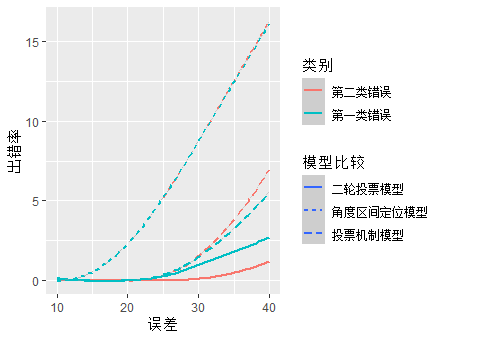
\includegraphics[width=0.60\linewidth]{pic/三类比较.png}
    \caption{三种模型报错概率折线图}
    \label{三种模型报错概率折线图}
\end{figure}

不难看出二轮投票模型的报错率明显低于其他两个模型,甚至能够在计算出的发射点不完全正确的情况下得出正确的定位信息(数据表现为第一类错误率大于第二类错误率),模型优化效果明显。

在模拟时,我们也记录了两种判断定位失败的方法判断的结果,发现在所有模拟中两种方法计算得出的定位失败率都相同,故可以证明用角度判断定位准确度的正确性。(具体结果可以查看支撑文件)











\end{document}